\documentclass[11pt]{article}
\usepackage[margin=2.6cm]{geometry}
\usepackage{graphicx,booktabs,amsmath,microtype,array}
\usepackage{float}   % [H]: figures stay where they are written
\usepackage[round,authoryear]{natbib}
\usepackage[hidelinks]{hyperref}
\usepackage[dvipsnames]{xcolor}
\graphicspath{{figures/}}
\newcommand{\code}[1]{\texttt{\small #1}}
\setlength{\parskip}{4pt}\setlength{\parindent}{0pt}
\title{The empirical construction\\[2pt]
\large The health measure and the cost index: what they are made of, how they are built, and what they deliver}
\author{Julian Ashwin}
\date{September 2026}

\begin{document}
\maketitle

\noindent Part~I is the health measure, built by \code{data\_cleaning/04\_build\_health.py} over
\code{measures/health.py}, with figures and the properties table from
\code{descriptives/21\_health\_measure.py}. Part~II is the cost index, built by
\code{data\_cleaning/05\_build\_cost\_proxy.py} and validated by
\code{descriptives/15}--\code{17}; the mortality and correlation figures come from \code{descriptives/24\_paper\_measure\_tables.py}. Every number below is printed by those scripts. Cost is in pounds throughout: convexity of cost in health is already the non-linearity the framework is about, and a log or proportional gradient would change the estimand away from mean cost. The search that
chose the measure among 85 candidates is archived in \code{health\_measures\_note.tex} and
\code{redo\_concepts/baseline\_measure\_comparison.xlsx}.

\tableofcontents

\part{The health measure}

\section{The measure for an economics reader}
\label{sec:econ}

\subsection{What it is}
\begin{itemize}
\item One number per person-year for physical health, built from eight ordinal answers in UKHLS that every respondent gives every wave: four SF-12 physical items (self-rated general health, physical functioning, role limitations from physical health, bodily pain), three counts of impairment areas (functional: mobility, lifting, dexterity, co-ordination; self-care; sensory), and a count of ever-diagnosed physical conditions.
\item The scoring model is the graded-response model \citep{samejima1969}, the item-response-theory form of a one-factor model for ordinal indicators; with continuous indicators the same model is the linear factor model economists use (Section~\ref{sec:factor}). It estimates, for each item, how strongly it loads on latent health and where along the health scale each of its categories switches on; a person's score is the posterior mean of latent health given their eight answers.
\item The economist's translation: it is a factor score with weights the data chose. Regressing $h$ on the eight standardised item codes gives $R^2 = 0.993$, with about 70\% of the weight on the SF-12 items, 23\% on the impairment counts and 6\% on diagnoses (Appendix~\ref{sec:weights}). The deficit index is an exact linear function of the same codes; $\theta$ is not, at $R^2 = 0.925$, because the posterior mean stretches the tails where the bank carries least information. So on the $[0,1]$ scale the model's practical content is the weighting rather than the functional form; on the latent scale the functional form does some work too.
\end{itemize}

\subsection{Why not something off the shelf}
\begin{itemize}
\item The SF-12 physical component summary (PCS) is the obvious alternative and correlates at $0.90$--$0.94$ with ours, but its weights were chosen in a 1990s US general-population sample to reproduce the SF-36 summaries \citep{ware1996}, whose orthogonal factor structure puts weight on the mental-health items too \citep{farivar2007}, and it has a hard floor: the very sick pile up at the worst score. Our bank has 7 person-waves in the whole 60--84 sample at the worst attainable value, against 1.1\% for a functioning-only bank; the diagnosis count keeps separating people after every functioning item has bottomed out.
\item The floor matters because prevention is a question about the sick tail, and because healthcare cost is convex in health: the region where alternative measures stop resolving is the region that carries the cost.
\item A single chronic-condition count, the other common choice, is monotone by construction and cannot fall, so it carries no information about recovery or persistence.
\end{itemize}

\subsection{Three versions of the same score}
\begin{itemize}
\item $\theta$: the latent scale, standard normal in the pooled sample. A $\theta$ of $-1$ means the same latent health at 30 as at 80, because the age profile is estimated separately and does not feed back into scores. This is the default scale for the dynamic models, which are also fitted on $h$ and the deficit index.
\item $h$: $\theta$ pushed through the model's expected-score curve onto $[0,1]$, the share of the bank's total scale a person is expected to answer at. Monotone in $\theta$, so identical rankings, but not affine: the curve is flat at the healthy end and steep among the sick, so a standard deviation of $h$ is much less health among the healthy than among the sick. This is the $[0,1]$ health variable the framework's cost function is written on.
\item The ten-deficit index: the same answers pooled with equal weights, one minus the mean deficit, in the frailty-index tradition \citep{mitnitski2001,searle2008}. Computable by hand from the questionnaire, 121 distinct values, Spearman $0.99$ with $h$, and it reaches the same conclusions everywhere $h$ does.
\end{itemize}

\subsection{What the scale choice does and does not change}
\begin{itemize}
\item Anything that is a rank statistic is invariant: correlations with the PCS, the MCS and the condition count, the mortality gradient by decile, the ordering of people, the out-of-sample prediction of death and utilisation.
\item The cost conclusions hold on every ruler. Cost in pounds is convex in health on all of them, and at a fixed level of health it barely moves with age: the health-by-age interaction is insignificant on every variant (Section~\ref{sec:invariance}). What the ruler changes is magnitudes. The convexity per standard deviation is two to three times as large on $\theta$ as on $h$, and the pound gradient per standard deviation is steeper among the young on $h$, because a standard deviation of $h$ is more health among the healthy.
\item Where the ruler matters is the distribution of health and its dynamics. Variance by age keeps rising to the top of the age range on $h$ and turns over in the early sixties on $\theta$, and on $h$ the ceiling breaks a Gaussian dynamic model for the healthiest class (Section~\ref{sec:factor}).
\item The typology is scale-dependent in a specific way: on $h$ and the deficit index a 10\% sick tail separates; on $\theta$ the healthy majority splits. Clustering methods agree within a scale and disagree across scales.
\end{itemize}

\subsection{Validation, in one line each}
\begin{itemize}
\item Mortality: the log-odds of dying before the next wave fall by $0.85$ per standard deviation of $\theta$; the death rate in the least healthy decile is 43--45 times that in the healthiest.
\item Utilisation: the cost index of Part~II rises with poor health at an increasing rate on every variant, and the sickest decile costs 10--14 times the healthiest at every age.
\item Measurement error: once a one-period error is allowed in the dynamic model, between a fifth and a half of the variance around each type's trajectory on $\theta$ is measurement error (signal shares $0.78$, $0.63$ and $0.56$ across the three types), and the score's own noise scale ranks the instruments: the diagnosis items make it less noisy, not more.
\end{itemize}

\subsection{The honest caveats}
\begin{itemize}
\item Self-reported throughout, including diagnoses; no administrative linkage yet.
\item A ceiling: 7\% of person-waves give the best answer to all eight items, and on the bounded $h$ scale that ceiling is what breaks a Gaussian dynamic model for the healthiest class.
\item Physical only, by design; mental health is a separate bank with a correlation of $0.46$ to this one.
\end{itemize}

\subsection{Relation to the economics literature}
\label{sec:lit}

\noindent\emph{Section, table and page references below were checked against the papers (working-paper versions where the published text was not accessible); page numbers follow the version named.}

\paragraph{Health as a latent index.}
\begin{itemize}
\item Economists who need one health variable have mostly built it by factor methods from many indicators. \citet{poterba2013,poterba2017} take the first principal component of 27 HRS items covering self-reported health, diagnoses, ADLs and IADLs (2013, Section~2 and Table~2-1). \citet{blundell2023} extract one index as the first principal component of the three subjective health measures common to HRS and ELSA, test the single-index assumption against the full set of ten diagnosed conditions (working paper, Section~3.4), and conclude that a single index captures the employment-relevant variation in health. A first principal component approximates a one-factor model fitted as if the items were continuous, so these indices are close relatives of ours. Our measure belongs to that tradition, with the ordinal factor model fitted properly rather than a principal component of mixed-type items, and with its weights reported (Appendix~\ref{sec:weights} is written for exactly that reader).
\item The nearest thing in economics to what the measurement model does is \citet{cunha2010} on skill formation. They estimate a dynamic factor model on 2,207 children of the NLSY/79: each PIAT test score and Behavior Problem Index subscale is a loading on the log of a latent cognitive or noncognitive skill plus error, the joint distribution of the latents is identified nonparametrically from two measures per factor with error that may be nonclassical, and a {CES} technology then maps skills, parental investment and parental skills into next period's skills (Sections~3 and~4.1). Because a latent factor is identified only up to a monotone transformation --- ``any monotonic function of a test score is a valid test score'' (p.~890) --- they anchor the scale by estimating its effect on an adult outcome with natural units, years of schooling attained, and report that anchoring changes the estimates while nonnormality of the factors barely does (Section~3.5; \citealp{cunha2008}).
\item Their measurement system and ours are the same model applied to different data. A one-factor model with a loading per measure is what the graded-response model becomes when the indicators are continuous: the threshold layer drops out and each measure is linear in the factor plus error. With ordered categories the same factor model needs thresholds, and the graded-response model is its item-response form \citep{takane1987}. So the difference is the data, and it has consequences. Their measures are continuous test scores, linear in the log of the latent skill, so their identification results and their nonparametric treatment of nonclassical error apply directly. Ours are ordinal items with a handful of categories, where a loading on a level is not defined and the spacing between categories is itself a parameter: that is what the graded-response model estimates, and it is why we cannot simply transplant their measurement system. The compensation is that item-response models for exactly these items are already validated in the health-measurement literature, the PROMIS physical-function bank of 124 items being calibrated with the same graded-response model \citep{cella2010}. We also stop short of their second stage: we estimate the measurement model and describe the dynamics, with no production function and no investment.
\item The frailty or deficit-accumulation index from gerontology, the proportion of a list of deficits a person has \citep[92 items in the original;][]{mitnitski2001}, with equal weights acknowledged as a deliberate simplification \citep{mitnitski2002} and a recommended minimum of ``at least 30--40'' deficits \citep[Discussion]{searle2008}, has been imported into economics by \citet{hosseini2022}, who build one from 28 deficits in the PSID 2003--2017 (Section~2), and by \citet{abeliansky2018,abeliansky2019} in SHARE, where deficits rise by about 2.5\% a year of age (2018, Section~2.2) and fall by 1.4--1.5\% a year of later birth. Our ten-deficit index is the same idea on UKHLS items, with one departure that matters: the impairment areas are grouped before averaging, because the ungrouped version is concave in cost.
\item \citet{hosseini2022} also give the closest published counterpart to our stochastic specification: for people with positive frailty, log frailty is an individual fixed effect plus an AR(1) plus a white-noise term ``capturing both measurement error and acute health events'' (Section~4.1, eqs.~4--6), with a separate probit for the 15\% of observations at zero frailty (Section~4.1.1, Table~1), estimated by simulated method of moments on the autocovariance profiles, with $\rho=0.991$ (Table~9). That is our AR(1) plus measurement error structure, and our persistence near one, found in a different survey with a different index.
\end{itemize}

\paragraph{Item response models in economics.}
\begin{itemize}
\item Item response models are used in economics, but they cluster in two places, and health is not one of them. The first is the measurement of learning, where the problem is to put scores from different tests, years or countries on one scale. \citet{dashammer2005} measure clinical competence from vignette responses with a three-parameter logistic model (working paper, Section~3 and eq.~1); \citet{daszajonc2010} put two Indian states onto the TIMSS 1995 scale with a three-parameter model whose item parameters are fixed at the published TIMSS values, and give a methods appendix written for economists (working paper, Section~2 and Appendix~A, covering maximum-likelihood scores, expected a posteriori scores and plausible values). The same scaling is standard in applied work downstream: \citet{muralidharan2019} score their experimental tests with a three-parameter model linked by common items (online appendix, Sections~E.4--E.5), \citet{singh2020} with a three-parameter model for multiple-choice items and a two-parameter model for open-response ones, linked across countries within an age group and explicitly not across ages (accepted manuscript, Appendix~B and the note to Table~2), and \citet{andrabi2011} use item-response-scaled scores as the input to value-added estimation, the model being named only in the earlier working paper \citep[footnote~14]{andrabi2008}.
\item The second cluster is the one we are closer to: a bank of ordinal or binary survey items that has to become one number, in deprivation, food security, empowerment and financial literacy. \citet{moffitt2016} fit a Rasch model to eight food-hardship items in the Three City Study, imposing a single dimension rather than establishing one, and report that a likelihood-ratio test rejects equal discrimination while leaving the substantive results unchanged. \citet{farcomeni2025} build a material-deprivation scale from eight binary EU-SILC items by conditional maximum likelihood on the Rasch model, and argue for it over more flexible alternatives on the ground that raw scores stop being sufficient statistics once discriminations differ (Section~2.3). \citet{vollmer2022} use one- and two-parameter models, a Mokken procedure and classical test theory to select and validate the assets items of the global Multidimensional Poverty Index, though the published indicator remains counting-based. \citet{kaiser2026} fit a two-parameter model to the ``Big Three'' financial-literacy questions, chosen over one-, three- and four-parameter and multidimensional alternatives on fit, and find the short index performs much like the longer one.
\item Graded-response models specifically, the model we use, appear in four of these. \citet{corsini2020} apply Samejima's model to Italian EU-SILC living-conditions items screened by a Mokken procedure, and find the most informative items are the inability to afford a week's holiday, the inability to meet an unexpected expense and difficulty making ends meet (working paper, Sections~2--3). \citet{davis2026} replace the one-parameter model behind the official USDA food-security scale with a Bayesian graded-response model with a probit link and item-specific error variances, and conclude that there is substantial latent variation within the official categories and non-trivial overlap across them (working paper, Section~2 and Conclusion). \citet{yount2019} use a graded-response model for the ordered items of the project-level Women's Empowerment in Agriculture Index alongside two- and nominal-response models elsewhere, with the honest finding that the assumptions hold for only one item set (Section~3.3, Table~1).
\item In health the model is much rarer. The closest published counterpart to what we do is \citet{graeber2023}, who scores a latent health index from five SOEP items --- self-rated health, satisfaction with health, doctor visits, hospital visits and degree of disability --- with Samejima's graded-response model and empirical Bayes (Section~2.1; Appendix~B, eqs.~A13 and~A15), choosing it ``simply because of the finite scale of our items'' (footnote~3). \citet{wallace2017} build a health index from 21 RAND HRS items by marginal maximum likelihood in an item-response framework, without naming the parametric form. And \citet{meijer2011} estimate, on SHARE wave~1, what is mathematically an ordinal factor model with probit thresholds on binary and ordered health items --- the same object --- while calling it a LISCOMP or MIMIC model and never using the words item response (Section~3); grip strength anchors their scale for cross-country comparability, which is the anchoring move of \citet{cunha2008} applied to health.
\item Two lessons from that literature bear directly on this note. First, aggregation is not innocent: \citet{singh2015} reports that replacing item-response scores with normalised raw percentage-correct scores roughly halves his estimated private-school effect, from 0.66 to 0.32 standard deviations, and writes that equal weighting of questions understates it (accepted manuscript, Section~4, Table~4 and Appendix Table~A.2). Second, the step from the model to a usable score is where economists come unstuck: \citet{jacob2016} warn that test scales generally have no basis for an interval interpretation (p.~89), that posterior-mean scores carry error correlated with true ability so classical corrections fail (pp.~98--102, Tables~1--2), and that plausible values are neither unbiased estimators nor unbiased predictors (p.~96); \citet{jerrim2017} show on PISA that the imputation behind plausible values can overturn a pupil fixed-effects result, though averaging over plausible values itself changes little and survey weights move estimates more (working paper, Tables~3 and~6).
\item The question those lessons raise for us is whether the choice between an item-response score and a factor or principal-component score matters. \citet{graeber2023} states the expectation that it does not, in a footnote and without a comparison (footnote~3), and \citet{poterba2013} and \citet{blundell2023} take principal components without raising it. We answer it on our own bank rather than assume it: $h$ is a weighted sum of the eight coded answers to $R^2 = 0.993$ and the deficit index is an exact linear function of them, so on the bounded scale the model's content is the weighting and not the functional form (Appendix~\ref{sec:weights}). A linear factor score fitted directly to the codes correlates $0.998$ with that weighted sum and $0.992$ in rank with $\theta$ (Section~\ref{sec:factor}). Where the choice does bite is $\theta$, at $R^2 = 0.925$, and that is the scale on which the variance profile and the dynamics behave differently (Section~\ref{sec:factor}) --- so the honest version of Graeber's footnote is that the expectation holds on the bounded score and fails on the latent one.
\item The skill-formation literature uses the nearest relative of our model. Its linear factor model is the graded-response model for continuous measures: the same one-factor structure with a loading per measure, without the thresholds. \citet{attanasio2020} write each measure in levels as a linear function of the \emph{log} of the latent factor plus additive error, the log form chosen to keep the factors positive (Section~II.B, eqs.~2--4 and footnote~11, p.~57), with scale fixed by setting the first loading to one and location by normalising the control group's mean log factor to zero; several of their measures are plainly ordinal rating scales (Table~1, p.~59), and the ordinality of measures is raised once, in a footnote citing \citet{nielsen2015}, never about their own (footnote~16, p.~58). \citet{agostinelli2025} use the same log-linear system (Section~3.1, eq.~4) and are explicit about the cost: measures of child skills ``are fundamentally ordinal'' and the log-linear model ``does impose a kind of cardinality on the measures'' (working paper, p.~7), an issue they set aside because their subject is comparability across periods --- itself a warning, since they show elsewhere that re-normalising each period restricts the admissible technology to the Cobb--Douglas sub-class \citep[Remarks~1--2]{agostinelli2016}. Fitted to our ordinal codes as if they were continuous, that linear model orders people as ours does but lands with $h$, not $\theta$, on every scale-dependent property (Section~\ref{sec:factor}).
\item \citet{cunha2021} is the review that states the problem in the form we have to answer: its Section~2 is titled ``Cardinality'' and argues that psychometric scales are not cardinal, and its Section~3.1 is on item response theory, whose normalisation it treats as itself an arbitrary cardinalisation rather than an escape from one. That is the reason this note reports $\theta$ and $h$ side by side and does not pick one. It is also why the ordinal-robustness results belong here: \citet{nielsen2015} bounds how far achievement-gap statistics can move under order-preserving rescalings and finds gap \emph{trends} fragile, and \citet{domicolo2022} show the greater-male-variability finding reverses under plausible rescalings. Our $\theta$-against-$h$ comparison is the same exercise carried out on a health measure, with the variance profile, the dynamics and the size of per-standard-deviation cost effects as the statistics at risk. Whether cost in pounds is convex and age-invariant at fixed health turns out not to be at risk.
\end{itemize}

\paragraph{Self-reported health and its dynamics.}
\begin{itemize}
\item The workhorse of the health-dynamics literature is five-category self-assessed health, usually collapsed: to three states in the PSID by \citet[Section~2.1]{denardi2025} and in MEPS by \citet[Section~4.1]{capatina2015}, to a bad-health indicator in the PSID by \citet[Section~2]{halliday2008}, and kept categorical in the BHPS by \citet{contoyannis2004}, whose dynamic panel ordered probits find ``strong positive state dependence'' with heterogeneity ``around 30\% of the unexplained variation in health'' (abstract). \citet{denardi2025} add three fixed unobserved health types to a history-dependent transition model (Section~2.3) and find that the types ``account for more than 70\% of the variation of the fraction of lifetime spent in bad health'' (Section~1); \citet{halliday2008} finds near-unit state dependence for half the population (abstract, Tables~4--5). That is the same structure, persistence plus permanent heterogeneity, that our identification cases and the AR(1) plus measurement error mixture find; those papers get it from a single ordinal item with a floor of one category, and our bank exists to remove that floor. The general-health item of the SF-12 is self-assessed health, so our score nests theirs as one of eight items.
\item The reliability of self-reports is an old worry. \citet{bound1991} argues that self-reports ``may not be independent of the labor market outcomes we may wish to use them to explain'' and that measurement error and this endogeneity bias the estimated effect of health in opposite directions, so the two kinds of measure bound it (working paper, pp.~1--2 and 16--17). \citet{crossley2002} find that 28\% of respondents change their self-assessed health when asked a second time within the same interview, 3\% by more than one category (abstract; working paper, Section~4). \citet{baker2004} link the 1994 Canadian National Population Health Survey to Ontario claims records and find that for many conditions over half of those with a recorded diagnosis do not report it, with reporting-error variance between 30\% and 80\% of the total (abstract; Table~3a). \citet{kapteyn2007} use vignettes to show that most of the US--Dutch gap in reported work disability is a difference in reporting thresholds (abstract). Our measurement-error estimates speak to that literature directly: a fifth to a half of the variance around each type's trajectory is one-period noise, and adding the diagnosis items reduces it.
\item \citet{idler1997} review 27 community studies and find self-rated health an independent predictor of mortality ``in nearly all of the studies'' after clinical covariates (abstract); our mortality gradient by decile is the same validation on the composite.
\end{itemize}

\paragraph{Scale and cardinalisation.}
\begin{itemize}
\item \citet{bond2013,bond2019} make the point, for test scores and for happiness scales, that an ordinal measure identifies rankings and nothing more: any monotone transformation is an admissible scale, so statements about means, gaps or changes in gaps can be reversed by re-scaling (2013, Sections~1--2; 2019, Section~2.2, where a lognormal transformation reverses an ordered-probit ranking, and the conclusion that two groups can be ranked only under first-order stochastic dominance). Our $\theta$ versus $h$ contrast is that point in health: identical rankings, a variance profile that keeps rising to the top of the age range on one ruler and turns over in the early sixties on the other, and per-standard-deviation cost effects of different sizes. The response of \citet{cunha2008}, to anchor the latent scale to an outcome with natural units, is available to us in principle: the cost index of Part~II is the natural candidate anchor, being in pounds and being the quantity the framework's cost function is about. We do not take that step here. We report both scales instead. In pounds the cost conclusions turn out not to depend on the choice (Section~\ref{sec:invariance}), while the distributional and dynamic ones do (Section~\ref{sec:factor}); an anchored scale would be a natural extension, and would have to confront the fact that the anchoring regression is itself estimated on the scale in question.
\item The choice of ruler is not cosmetic for dynamics either. The frailty index of \citet{hosseini2022} is bounded like $h$; they model its logarithm, and our finding that a Gaussian dynamic model in levels breaks at the ceiling on $h$ is a warning that carries over to any bounded health index used in a linear state-space model.
\end{itemize}

\paragraph{Cost, convexity and the health--cost link.}
\begin{itemize}
\item The steep rise of medical spending in age and its concentration among the sick is the mechanism in \citet{denardi2010} on precautionary saving by the elderly: out-of-pocket expenses rise from \$1,100 at 75 to \$9,200 at 95 (Introduction; Figure~3 by age and permanent income) and are about 50\% lower for the healthy conditional on age, sex and income (p.~53). \citet{finkelstein2013} add that the marginal utility of consumption itself falls as health deteriorates, by 10--25\% per standard deviation of chronic conditions (Table~2). Our contribution is to estimate the shape of cost in health on a scale that resolves the sick tail, and to show it is close to age-invariant conditional on health.
\item The earnings-dynamics literature is the template for reading permanent, persistent and transitory components off a covariance surface: \citet[Section~3.2, eq.~5]{meghir2004} identify the permanent-shock variance from autocovariances of income growth, \citet[Section~4]{guvenen2009} from the age structure of variances and autocovariances, and \citet[Section~III.B]{blundell1998} the same components from the joint growth of consumption and income variances in repeated cross-sections. Guvenen's distinction between heterogeneous income profiles (individual-specific slopes with modest shock persistence) and restricted profiles (a common slope with very persistent shocks) is precisely our question of types against a persistent state; the framework note's identification section is that machinery applied to health, and its Exhibit~2 is the health analogue of a covariance-structure decomposition.
\end{itemize}

\section{The measure in one page}

The project needs one number per person-wave saying how healthy someone is
\emph{physically}, on a scale where being sicker costs more at an increasing
rate, where the very unwell are not all bunched at a floor, and where the
answer does not turn on how the scale happens to be cardinalised. That number
is fitted to eight ordinal items from UKHLS:

\begin{center}\small
\begin{tabular}{llc}
\toprule
Item & What it records & Categories \\
\midrule
GH & self-rated general health (\code{sf1}) & 5 \\
PF & moderate activities and climbing stairs (\code{sf2a}, \code{sf2b}) & 5 \\
RP & accomplished less, limited in kind of work (\code{sf3a}, \code{sf3b}) & 9 \\
BP & pain interference with normal work (\code{sf5}) & 5 \\
LIM\_FL & functional limitations: mobility, lifting, dexterity, co-ordination & 5 \\
LIM\_SELF & self-care: personal care, continence & 3 \\
LIM\_SENS & sensory: hearing, sight & 3 \\
COND & ever-diagnosed physical conditions, 0--5 and 6 or more & 7 \\
\bottomrule
\end{tabular}
\end{center}

The first four are the SF-12 physical testlets already validated for this
project; the next three count the UKHLS impairment areas, grouped; the last
counts diagnoses. In the search's notation this bank is \textbf{P-LIM3+CC}.
The sample is \textbf{387{,}599 person-waves} on \textbf{69{,}958 people},
waves 1--15, ages 20--90, complete on all eight items --- 5.5 observations per
person on average.

A graded-response model turns the eight answers into a latent health score.
The measure is reported three ways, all monotone in the same answers:

\begin{center}\small
\begin{tabular}{llp{8.4cm}}
\toprule
 & Scale & What it is \\
\midrule
$\theta$ & standard normal in the pool & the latent score, expected a posteriori \\
$h$ & $[0,1]$, here $0.11$ to $0.98$ & $\theta$ through the expected-score curve: the share of the bank's total scale a person is expected to answer at \\
\code{fi10} & $[0,1]$, $1$ = no deficits & a ten-deficit index: the six SF-12 physical items graded by response step, the three impairment groups as the share of their areas, and the condition count capped at six --- equal weights, computable by hand \\
\bottomrule
\end{tabular}
\end{center}

They rank people almost identically (Spearman $0.991$ between $h$ and
\code{fi10}) and they agree on every conclusion about cost: convex in health,
and close to age-invariant at a fixed level of health (section~\ref{sec:invariance}).
Where they differ is in magnitudes per standard deviation and in the
distribution of health: the variance profile by age, and how the healthiest
behave in a dynamic model (section~\ref{sec:factor}). $\theta$ is the default; $h$ is the scale the
framework's $[0,1]$ health variable maps to; \code{fi10} is the transparent
version a reader can reconstruct from the questionnaire.

\section{The variables and the coding rules}

\subsection{The SF-12 physical testlets}

Six SF-12 items enter as four testlets, the grouping validated in the archived
note: the two physical-function items sum into PF, the two role-physical items
sum into RP, and general health and pain enter alone. Summing the pairs is what
removes the positive local dependence between them --- the two items in each
pair share wording, and left separate their residual correlation would be read
as evidence of a second dimension. Every item is coded so category 1 is worst
health.

\subsection{The impairment areas}

UKHLS asks which of a list of areas a person's health limits them in. Eight are
physical and used here, in three groups:

\begin{center}\small
\begin{tabular}{lll}
\toprule
Group & Areas (\code{disdif} codes) & Count \\
\midrule
LIM\_FL & mobility (1), lifting (2), dexterity (3), co-ordination (10) & 0--4 \\
LIM\_SELF & continence (4), personal care (11) & 0--2 \\
LIM\_SENS & hearing (5), sight (6) & 0--2 \\
\bottomrule
\end{tabular}
\end{center}

Two coding rules hold throughout, and both are decisions rather than data.

\textbf{The routing rule.} In the early waves the battery was asked only of
people reporting a long-standing illness. Someone who reports none therefore
has no answer, not a zero. We count them as having no limitation, in every
wave, so that the variable means the same thing across the panel; someone who
does report a long-standing illness but has no usable answer is missing. The
alternative --- treating unrouted rows as missing --- would drop the healthy
half of the sample, and with it the part of the distribution where prevention
happens.

\textbf{The merge rule.} A top count category holding less than $0.5\%$ of
person-waves is merged into the one below, decided on the sample before any
model is fitted. This is what fixes LIM\_FL at five categories (0, 1, 2, 3, 4+)
and LIM\_SELF and LIM\_SENS at three. Categories thinner than that are
estimated off a few hundred people and their thresholds wander.

Two areas are deliberately left out. ``Recognising when in physical danger''
loads with the mental items, and the whole point of this measure is that it
carries no mental health. ``Other health problem or disability'' is
non-specific: added as its own group (the search's P-LIM3+O) it changes
nothing, and it is one more judgement call for no gain.

\subsection{The condition count}

COND counts the sixteen ever-diagnosed physical conditions in the UKHLS
inventory, 0 to 5 and 6 or more, the top category set by the merge rule on the
sample that has an inventory. It enters as one item, not as six clinical-group
items. Both versions were fitted. As six items the conditions take
$40\%$ of the weight in an unweighted index against $14.1\%$ in the model, so
the model version and the by-hand version stop agreeing --- which defeats the
purpose of having a by-hand version at all. As one count they take $6\%$ in the
model and $10\%$ in \code{fi10}, and the three variants stay interchangeable.

Requiring an inventory is what sets the sample: 387,599 person-waves rather
than the 497,423 that have SF-12 and limitations. That restriction is shared
with every condition-carrying candidate in the search, so it changes no
comparison, and it leaves the cost and mortality samples intact.

\subsection{Category use}

\begin{center}\small
\begin{tabular}{lr rrrrrrrrr}
\toprule
& $k$ & \multicolumn{9}{c}{share of person-waves, best category first (\%)} \\
\cmidrule(l){3-11}
GH & 5 & 13.29 & 33.33 & 31.71 & 15.58 & 6.10 & & & & \\
PF & 5 & 65.13 & 11.66 & 11.82 & 4.60 & 6.79 & & & & \\
RP & 9 & 52.18 & 6.85 & 12.77 & 4.55 & 11.57 & 2.68 & 4.76 & 1.20 & 3.44 \\
BP & 5 & 53.72 & 25.24 & 9.14 & 8.26 & 3.64 & & & & \\
LIM\_FL & 5 & 83.05 & 6.66 & 5.30 & 3.24 & 1.76 & & & & \\
LIM\_SELF & 3 & 94.15 & 4.74 & 1.12 & & & & & & \\
LIM\_SENS & 3 & 95.62 & 3.82 & 0.56 & & & & & & \\
COND & 7 & 48.28 & 28.88 & 12.90 & 5.59 & 2.44 & 1.05 & 0.86 & & \\
\bottomrule
\end{tabular}
\end{center}

$7.1\%$ of person-waves give the best answer to all eight items. That is the
measure's ceiling. It costs nothing for the cross-sectional questions, which
are asked at the other end, where 12 person-waves sit at the worst answer on
everything. It does matter for dynamics: on the bounded scales the ceiling is
what breaks a Gaussian dynamic model for the healthiest class
(Section~\ref{sec:factor}).

\section{The model}

\subsection{Graded response}

Item $j$ with $k_j$ categories has one discrimination $a_j$ and $k_j-1$
thresholds $b_{j1} < \dots < b_{j,k_j-1}$. The probability of answering at or
above category $c$ is logistic in $\theta$,
\[
P(Y_j \ge c \mid \theta) \;=\; \frac{1}{1 + \exp\{-a_j(\theta - b_{j,c-1})\}},
\]
and a single category's probability is the difference of adjacent curves. The
discriminations $a_j$ are on the logistic metric. Dividing $a_j$ by $1.702$
puts it on the normal-ogive (probit) metric, since a logistic curve with slope
$1.702$ is within $0.01$ of the standard normal distribution function
everywhere; that conversion is the source of the $1.702$ in
appendix~\ref{sec:weights}. The
model is Samejima's \citep{samejima1969}; its marginal likelihood is that of the ordinal factor model
\citep{takane1987}, which is where the weighted sum in appendix~\ref{sec:weights} comes from.

Estimation is marginal maximum likelihood by EM over distinct answer patterns
(28,360 of them), with the latent distribution identified as $N(0,1)$ in the
pooled sample and 121-point Gauss quadrature on $[-6,6]$. Fitting took 60 EM
iterations. Scores are expected a posteriori under the pooled prior, so a
$\theta$ means the same thing at every age --- the age profile is estimated
separately and does not feed back into anyone's score.

\begin{center}\small
\begin{tabular}{lrrl}
\toprule
Item & $k$ & $a$ & thresholds \\
\midrule
GH & 5 & 2.03 & $-2.10$\; $-0.98$\; $0.16$\; $1.45$ \\
PF & 5 & 3.52 & $-1.73$\; $-1.38$\; $-0.80$\; $-0.40$ \\
RP & 9 & 3.09 & $-2.20$\; $-2.03$\; $-1.56$\; $-1.37$\; $-0.81$\; $-0.64$\; $-0.23$\; $-0.03$ \\
BP & 5 & 2.31 & $-2.35$\; $-1.50$\; $-0.99$\; $-0.09$ \\
LIM\_FL & 5 & 3.38 & $-2.49$\; $-1.94$\; $-1.46$\; $-1.07$ \\
LIM\_SELF & 3 & 2.43 & $-2.95$\; $-1.99$ \\
LIM\_SENS & 3 & 1.36 & $-4.49$\; $-2.85$ \\
COND & 7 & 1.18 & $-4.61$\; $-3.90$\; $-3.12$\; $-2.26$\; $-1.25$\; $0.11$ \\
\bottomrule
\end{tabular}
\end{center}

The pattern is the one the measure was built for. PF, RP and LIM\_FL
discriminate hardest and their thresholds sit between $-2.5$ and $0$: they are
what separates people in the unhealthy half. GH and BP discriminate less but
reach further up, so they keep the healthy half from collapsing onto one point.
LIM\_SENS and COND discriminate least and sit furthest out --- they are the
items that keep the very sick from piling up at a floor, which is exactly the
job the archived search hired them for.

\subsection{Why the graded-response model and not the partial-credit one}

Both were fitted, on all six limitation banks. The graded-response model wins
by 13,500 to 15,200 log-likelihood points at equal parameter counts, every
time. The reason is structural: the generalised partial credit model makes a
weighted sum of category scores a sufficient statistic, which forces its steps
to be ordered in the data --- and PF and RP are sums of two items whose
categories are used very unevenly, so their steps are not. Their $\theta$s
correlate at $0.995$ and their clusters agree 97\% of the time, so nothing here
turns on the choice; the graded-response model is simply the better-fitting one.

\subsection{Local dependence}

Yen's $Q_3$ on the eight testlets has no positive off-diagonal above $+0.052$
(the expected value under the model is about $-1/(J-1) = -0.14$). Nothing in
the bank is measuring a second thing.

\subsection{The age profile}

Refitting multigroup by single year of age --- item parameters common across
ages, the pooled latent distribution standardised --- gives the latent mean and
standard deviation at each age. Mean health falls by $1.23$ pooled standard
deviations between 30 and 80, and the spread widens with age
(figure~\ref{fig:measure}c). These are descriptive: no score uses them.

\begin{figure}[H]
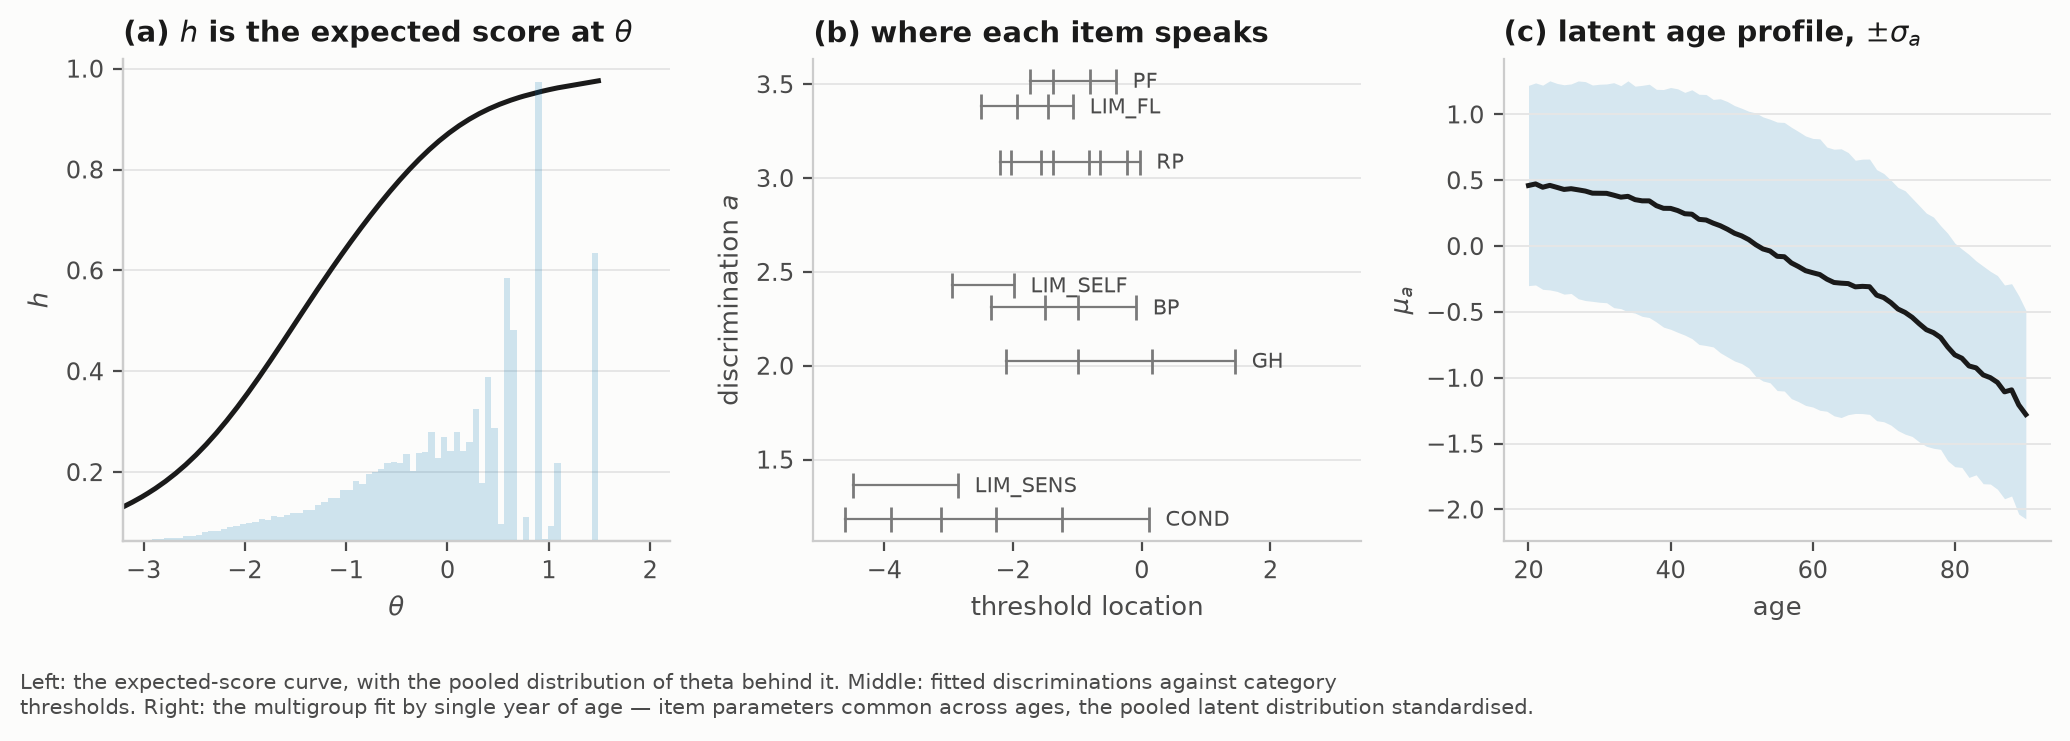
\includegraphics[width=\linewidth]{fig_health_measure}
\caption{The measure. (a) the expected-score curve that turns $\theta$ into
$h$, over the pooled distribution of $\theta$; (b) each item's discrimination
against the location of its thresholds; (c) the latent age profile.}
\label{fig:measure}
\end{figure}

\section{The three variants}

\subsection{$\theta$ and $h$}

$h$ is $\theta$ pushed through the test characteristic curve and rescaled to
$[0,1]$: the expected share of the bank's total scale. The map is monotone, so
$\theta$ and $h$ order people identically and no rank statistic can separate
them. It is not affine, and that is the whole of the difference between them:
the curve is flat at the top and steep in the middle (figure~\ref{fig:measure}a),
so a standard deviation of $\theta$ buys much less $h$ among the healthy than
among the sick. The size of anything reported per standard deviation --- a
cost gradient, a variance profile --- therefore depends on which of the two is
used. Sections~\ref{sec:invariance} and~\ref{sec:factor} set out which
conclusions survive the choice.

\subsection{The ten-deficit index}

\code{fi10} is the version that needs no model. Each of ten deficits is scored
between 0 and 1 and the index is one minus their mean, so 1 is no deficits:

\begin{center}\small
\begin{tabular}{lp{9.6cm}}
\toprule
6 deficits & the SF-12 physical items \code{sf1}, \code{sf2a}, \code{sf2b}, \code{sf3a}, \code{sf3b}, \code{sf5}, each graded 0 to 1 by response step \\
3 deficits & LIM\_FL, LIM\_SELF, LIM\_SENS as the share of their areas mentioned \\
1 deficit & the condition count, capped at six, divided by six \\
\bottomrule
\end{tabular}
\end{center}

This follows the deficit-accumulation tradition \citep{mitnitski2001,searle2008}, with one departure that is not cosmetic:
the impairment \emph{areas} are grouped before they are averaged. Scored area
by area, the eight areas would take more than half the index's weight and the
result stops being convex in cost --- on costs capped at the 99th percentile
the area version's cost curvature is $t = -2.0$ against $t = +12.0$ for the
grouped one. Equal
weights are defensible here only because the groups make the units comparable
first.

\code{fi10} takes 121 distinct values, against 28,360 for $\theta$. It is
coarser, not discrete in any way that matters: no value holds a large mass and
the bottom percentile alone is spread over 26 of them.

\begin{figure}[H]
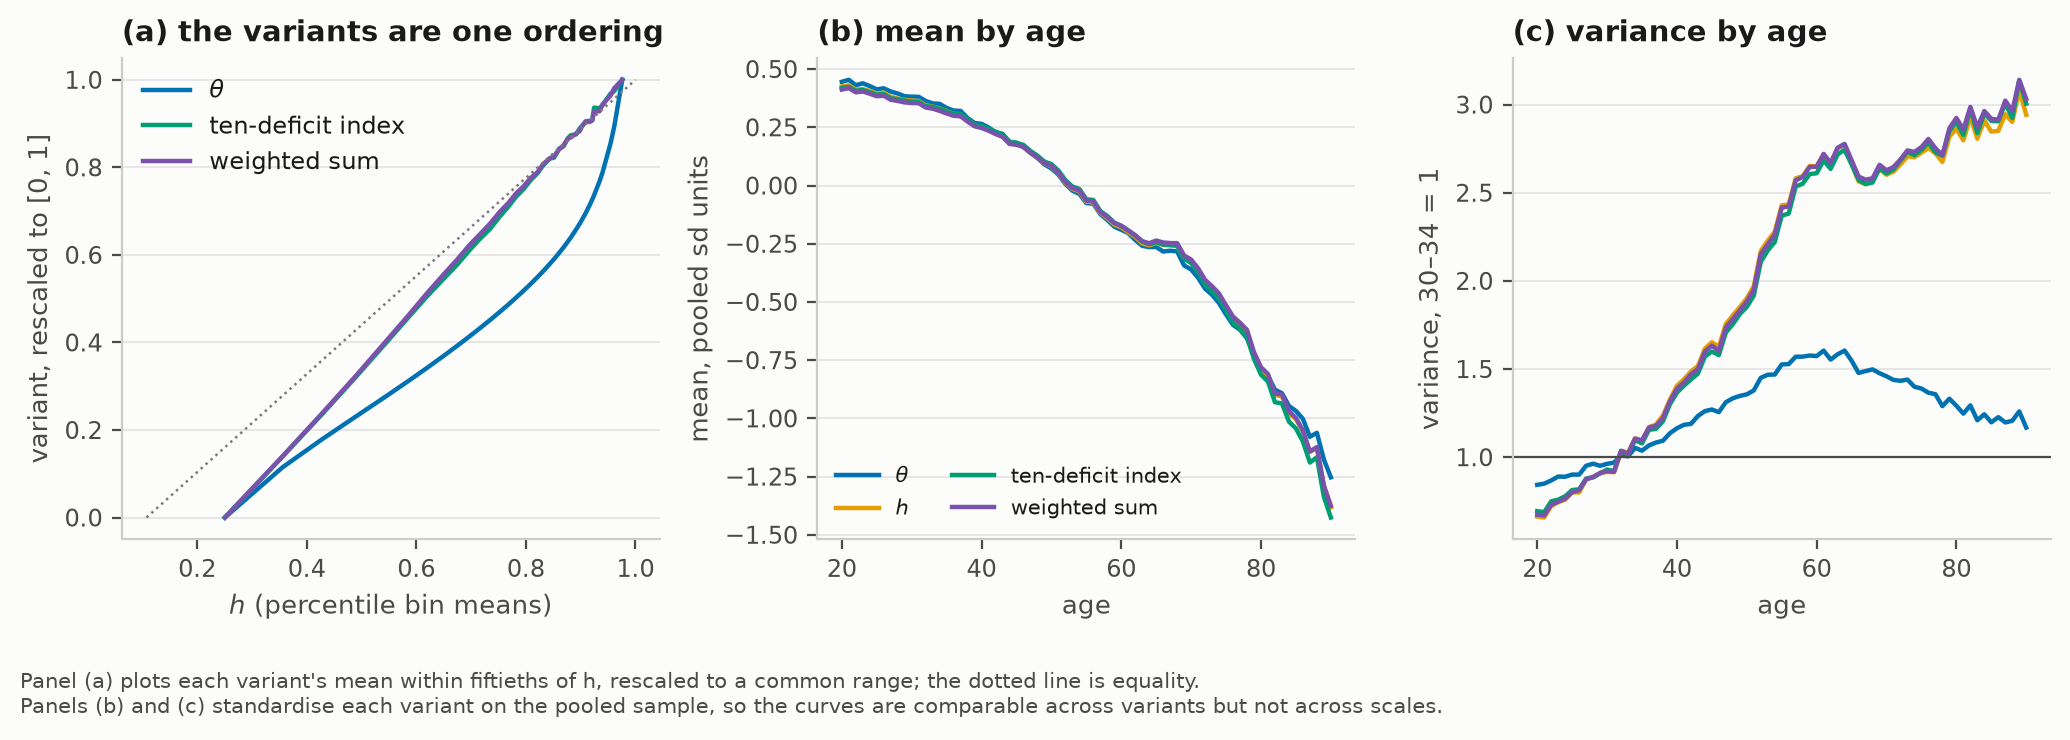
\includegraphics[width=\linewidth]{fig_health_variants}
\caption{The variants. (a) each variant's mean within fiftieths of $h$,
rescaled to a common range --- \code{fi10} and the weighted sum track $h$
almost exactly, while $\theta$ bends away because the map between them is not
affine; (b) and (c) mean and variance by age, each variant standardised on the
pooled sample.}
\label{fig:variants}
\end{figure}

\section{What the measure delivers}

The criteria below are the ones the search was run against; the archived note
has them for all 85 candidates.

\subsection{No floor, and no discreteness that bites}
\label{sec:floor}

\begin{center}\small
\begin{tabular}{lrrrrrr}
\toprule
 & distinct & at the worst & \multicolumn{2}{c}{variance ratio} & \multicolumn{2}{c}{cost curvature} \\
\cmidrule(lr){4-5}\cmidrule(l){6-7}
 & values & value, 60--84 & 30$\to$60 & 60$\to$85 & $\hat\gamma$ & $t$ \\
\midrule
$\theta$ & 28{,}360 & 7 & 1.62 & 0.77 & 105.5 & 36.9 \\
$h$ & 28{,}360 & 7 & 2.85 & 1.08 & 34.6 & 11.3 \\
\code{fi10} & 121 & 7 & 2.80 & 1.12 & 36.8 & 11.9 \\
weighted sum & 28{,}360 & 7 & 2.84 & 1.11 & 30.2 & 9.9 \\
\bottomrule
\end{tabular}
\end{center}

Seven person-waves in the whole 60--84 sample sit at the worst attainable
score --- $0.006\%$. The same share is $1.11\%$ for the functioning-only bank
the project used before, $0.10\%$ once the sensory and continence areas are
added and $0.023\%$ for the three-group version without conditions. The condition count is what
finishes the job: it keeps separating people after every limitation item has
bottomed out.

\subsection{Convexity in cost}

Cost rises with poor health at an increasing rate on every variant: the
quadratic term in the standardised measure is positive with $t$ between 9.9 and
36.9, person-clustered, on costs capped at the 99th percentile
(figure~\ref{fig:health_cost}). This is the criterion the whole search was
really about, and it is the one that fails for plausible-looking alternatives:
an ungrouped deficit index is \emph{concave}.

\begin{figure}[H]
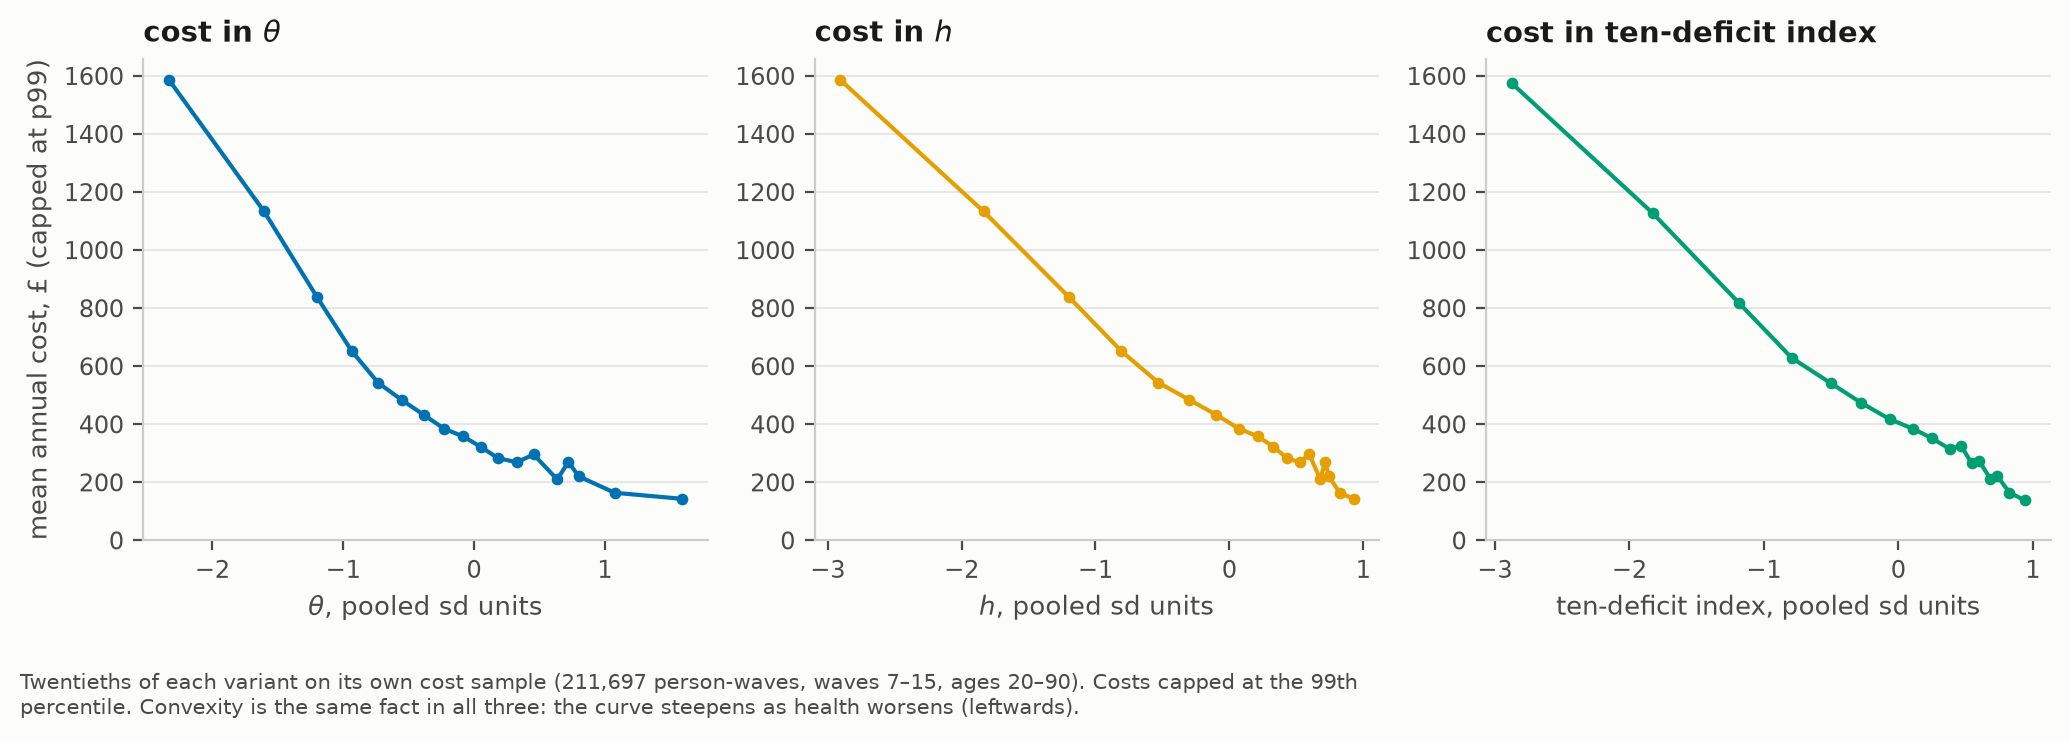
\includegraphics[width=\linewidth]{fig_health_cost}
\caption{Mean annual healthcare cost by twentieth of each variant. The curve
steepens as health worsens (leftwards) in all three.}
\label{fig:health_cost}
\end{figure}

\subsection{In pounds, age-invariance holds on every scale}
\label{sec:invariance}

The question is whether a given amount of poor health costs more at 80 than at 25. Over the full range the pound gradient per standard deviation rises with age on every variant, but that is mostly composition: cost is convex in health, and older people sit further into the steep part of the curve. $2.5\%$ of the 20--34 band is in the sickest pooled tenth, against $24.7\%$ of the 75--90 band. Three tests separate that from a change in the curve itself, all on the cost index in pounds.

\begin{center}\small
\begin{tabular}{lrrrrrr}
\toprule
 & \multicolumn{3}{c}{\pounds{} per sd sicker, full range} & common support & \multicolumn{2}{c}{health $\times$ age, $t$} \\
\cmidrule(lr){2-4}\cmidrule(lr){5-5}\cmidrule(l){6-7}
 & 20--34 & 75--90 & ratio & ratio, range & uncapped & capped \\
\midrule
$\theta$ & 357 & 741 & 2.07 & 0.88--1.41 & $-0.6$ & $-1.0$ \\
$h$ & 526 & 672 & 1.28 & 0.79--1.04 & $-0.3$ & $-1.7$ \\
\code{fi10} & 506 & 663 & 1.31 & 0.96--1.11 & $-0.6$ & $-1.5$ \\
weighted sum & 519 & 663 & 1.28 & 0.92--1.06 & $-0.2$ & $-1.2$ \\
\bottomrule
\end{tabular}
\end{center}

\begin{itemize}
\item \textbf{Cost at a fixed level of health.} In bins of the pooled health distribution, cost barely moves with age. In the sickest tenth mean cost is \pounds2{,}143 at 20--34 against \pounds2{,}136 at 75--90, while mean cost over everyone rises $2.6$-fold across the same span (\pounds374 to \pounds969). The bins are percentiles, so this test is the same on every ruler.
\item \textbf{The pooled interaction test.} Cost regressed on age, age squared, health, health squared and health $\times$ age, with standard errors clustered on the person. The quadratic in health absorbs the convexity, so the interaction asks whether the curve tilts with age. It does not, on any variant, capped or uncapped: no $t$ exceeds $1.7$ in absolute value, and the point estimates are a few pounds per decade against a gradient of several hundred.
\item \textbf{The slope on a common support.} Restricting to a window of the pooled distribution that every age band populates brings the ratio of the oldest band's slope to the youngest's close to one. It is fragile: single answer patterns hold up to 11\% of the sample, so where the window edge falls moves the young band's slope, and the table reports the range over windows from the 5th--95th to the 25th--75th percentile. Windows are defined on the pooled percentile of $\theta$, so they select the same people on every ruler.
\end{itemize}

The ruler does not change the conclusion, but it changes magnitudes. Per standard deviation, the young band's gradient is \pounds526 on $h$ against \pounds357 on $\theta$, because a standard deviation of $h$ is more health among the healthy. The common-support ratio is higher on $\theta$ than on $h$ in every window. So a statement about how much a standard deviation of health is worth in pounds is a statement about a ruler. A statement that the pound cost of a given state of health does not depend on age is not: it holds on every scale here. This is also why the framework's cost curve can be written without an age argument.

\subsection{Identification}

The framework's identification tests ask whether the covariance structure of
four ages two years apart can separate true health dynamics from measurement
error, and in particular whether $\mathrm{Corr}(H,d)$ follows the sign path the
model implies --- positive among the young, negative among the old. The tests
differ in what they assume the error looks like and in which moments they use:

\begin{center}\small
\begin{tabular}{lcccccc}
\toprule
 & \multicolumn{3}{c}{balanced moments} & \multicolumn{3}{c}{pairwise moments} \\
\cmidrule(lr){2-4}\cmidrule(l){5-7}
 & Case 2 & Case 3 & Case 4 & Case 2 & Case 3 & Case 4 \\
\midrule
$\theta$ & $\surd$ & $\surd$ & $\surd$ & $\surd$ & --- & $\surd$ \\
$h$ & $\surd$ & $\surd$ & $\surd$ & $\surd$ & --- & --- \\
\code{fi10} & --- & $\surd$ & $\surd$ & $\surd$ & --- & --- \\
weighted sum & $\surd$ & $\surd$ & $\surd$ & $\surd$ & --- & --- \\
linear factor score$^{a}$ & --- & $\surd$ & $\surd$ & $\surd$ & --- & --- \\
\bottomrule
\end{tabular}

\smallskip\footnotesize $^{a}$ The archived search's one-factor score on this bank, which correlates $0.999$ with the one in Section~\ref{sec:factor}.
\end{center}

Case 2 is AR(1) measurement error, Case 3 adds age-specific error variance,
Case 4 is AR(1) plus a one-period spike (evaluated at the best admissible
persistence). $\theta$ recovers the sign path under five of the six; every
variant recovers it under at least three, including Case 4, which is the most
permissive about what the noise can be. Case 3 on pairwise moments fails for
all 85 candidates in the search, this measure included --- it is a property of
that estimator, not of any measure.

\subsection{Mortality}

The log-odds of dying before the next wave fall by $0.85$ per standard
deviation of $\theta$ ($0.66$ on $h$ and on \code{fi10}), on 363,033
person-waves at risk and 1,825 deaths; the death rate in the least healthy
decile is 43 to 45 times that in the healthiest.

\subsection{A linear factor model lands with $h$}
\label{sec:factor}

The alternative an economist would reach for is a linear factor model: the one-factor measurement system of the skill-formation literature, fitted to the eight codes as if they were continuous. It is the graded-response model with the threshold layer removed. Each code becomes linear in the factor, so the loadings survive but adjacent categories are forced to be equally spaced. The fitted thresholds are not equally spaced. For seven of the eight items the widest gap between adjacent thresholds is 1.0 to 1.9 times the narrowest, and for RP, the nine-category testlet built from two items, it is 3.3 times.

Fitted by iterated principal axes and scored with regression weights, the one factor takes $52\%$ of the trace of the correlation matrix, with loadings from $0.33$ on the sensory count to $0.83$ on physical functioning. The score correlates $0.998$ with the weighted sum of appendix~\ref{sec:weights}, and its Spearman correlation is $0.992$ with $\theta$ and $h$ and $0.998$ with \code{fi10}. The linear model therefore orders people as the graded-response model does. The question is which cardinalisation it produces, and the answer is $h$'s:

\begin{center}\small
\begin{tabular}{lrrrrrr}
\toprule
 & best pattern, & skew & variance & variance & cost & health $\times$ \\
 & sd above mean & & peaks at & 30$\to$60 & curvature & age, $t$ \\
\midrule
$\theta$ & 1.63 & $-0.54$ & 64 & 1.62 & 105.5 & $-0.6$ \\
$h$ & 0.92 & $-1.57$ & 87 & 2.85 & 34.6 & $-0.3$ \\
\code{fi10} & 0.93 & $-1.57$ & 87 & 2.80 & 36.8 & $-0.6$ \\
weighted sum & 0.93 & $-1.61$ & 87 & 2.84 & 30.2 & $-0.2$ \\
linear factor score & 0.90 & $-1.73$ & 87 & 3.07 & 17.2 & $-0.3$ \\
\bottomrule
\end{tabular}
\end{center}

Cost curvature is the quadratic term in pounds per standard deviation squared, on costs capped at the 99th percentile, as in Section~\ref{sec:floor}; the interaction is the uncapped health $\times$ age test of Section~\ref{sec:invariance}. On the distributional columns the linear factor score is a twin of $h$. It is bounded because it is a weighted sum of bounded codes: the $7.1\%$ who give the best answer to all eight items sit at a wall $0.90$ standard deviations above the mean, against $1.63$ for $\theta$, and its variance keeps rising to the top of the age range. On cost it reaches the same conclusions as every other score: convex in pounds, most weakly at $t = 5.8$, and with no detectable health $\times$ age interaction. On the identification tests it recovers the sign path under three of the six, as \code{fi10} does.

Three consequences follow.
\begin{itemize}
\item Fitting it adds no third answer to the cardinalisation question. It lands on the bounded side with $h$, \code{fi10} and the weighted sum. The one score on the other side is $\theta$, and what produces $\theta$ is exactly the threshold layer the linear model drops.
\item In dynamics it would inherit the ceiling that breaks the Gaussian AR(1) plus measurement-error mixture for the healthiest class on $h$, and more severely, since its healthy mass is more skewed.
\item The transformation that does change the picture is the one \citet{hosseini2022} use on their frailty index: model the log deficit, $-\log(1-h)$. It has the same ranking, puts the best answer pattern $1.76$ standard deviations above the mean, has skew $-0.13$, and its variance peaks at 61, so in its distribution it behaves like $\theta$ rather than $h$. It is not one of the reported variants. \citet{hosseini2022} apply it to positive frailty only, with a separate probit for the 15\% of their observations at zero; on $h$ that problem does not arise, since the all-best pattern maps to a deficit of $0.024$, while on \code{fi10} it would, with 7.1\% at zero.
\end{itemize}

\begin{figure}[H]
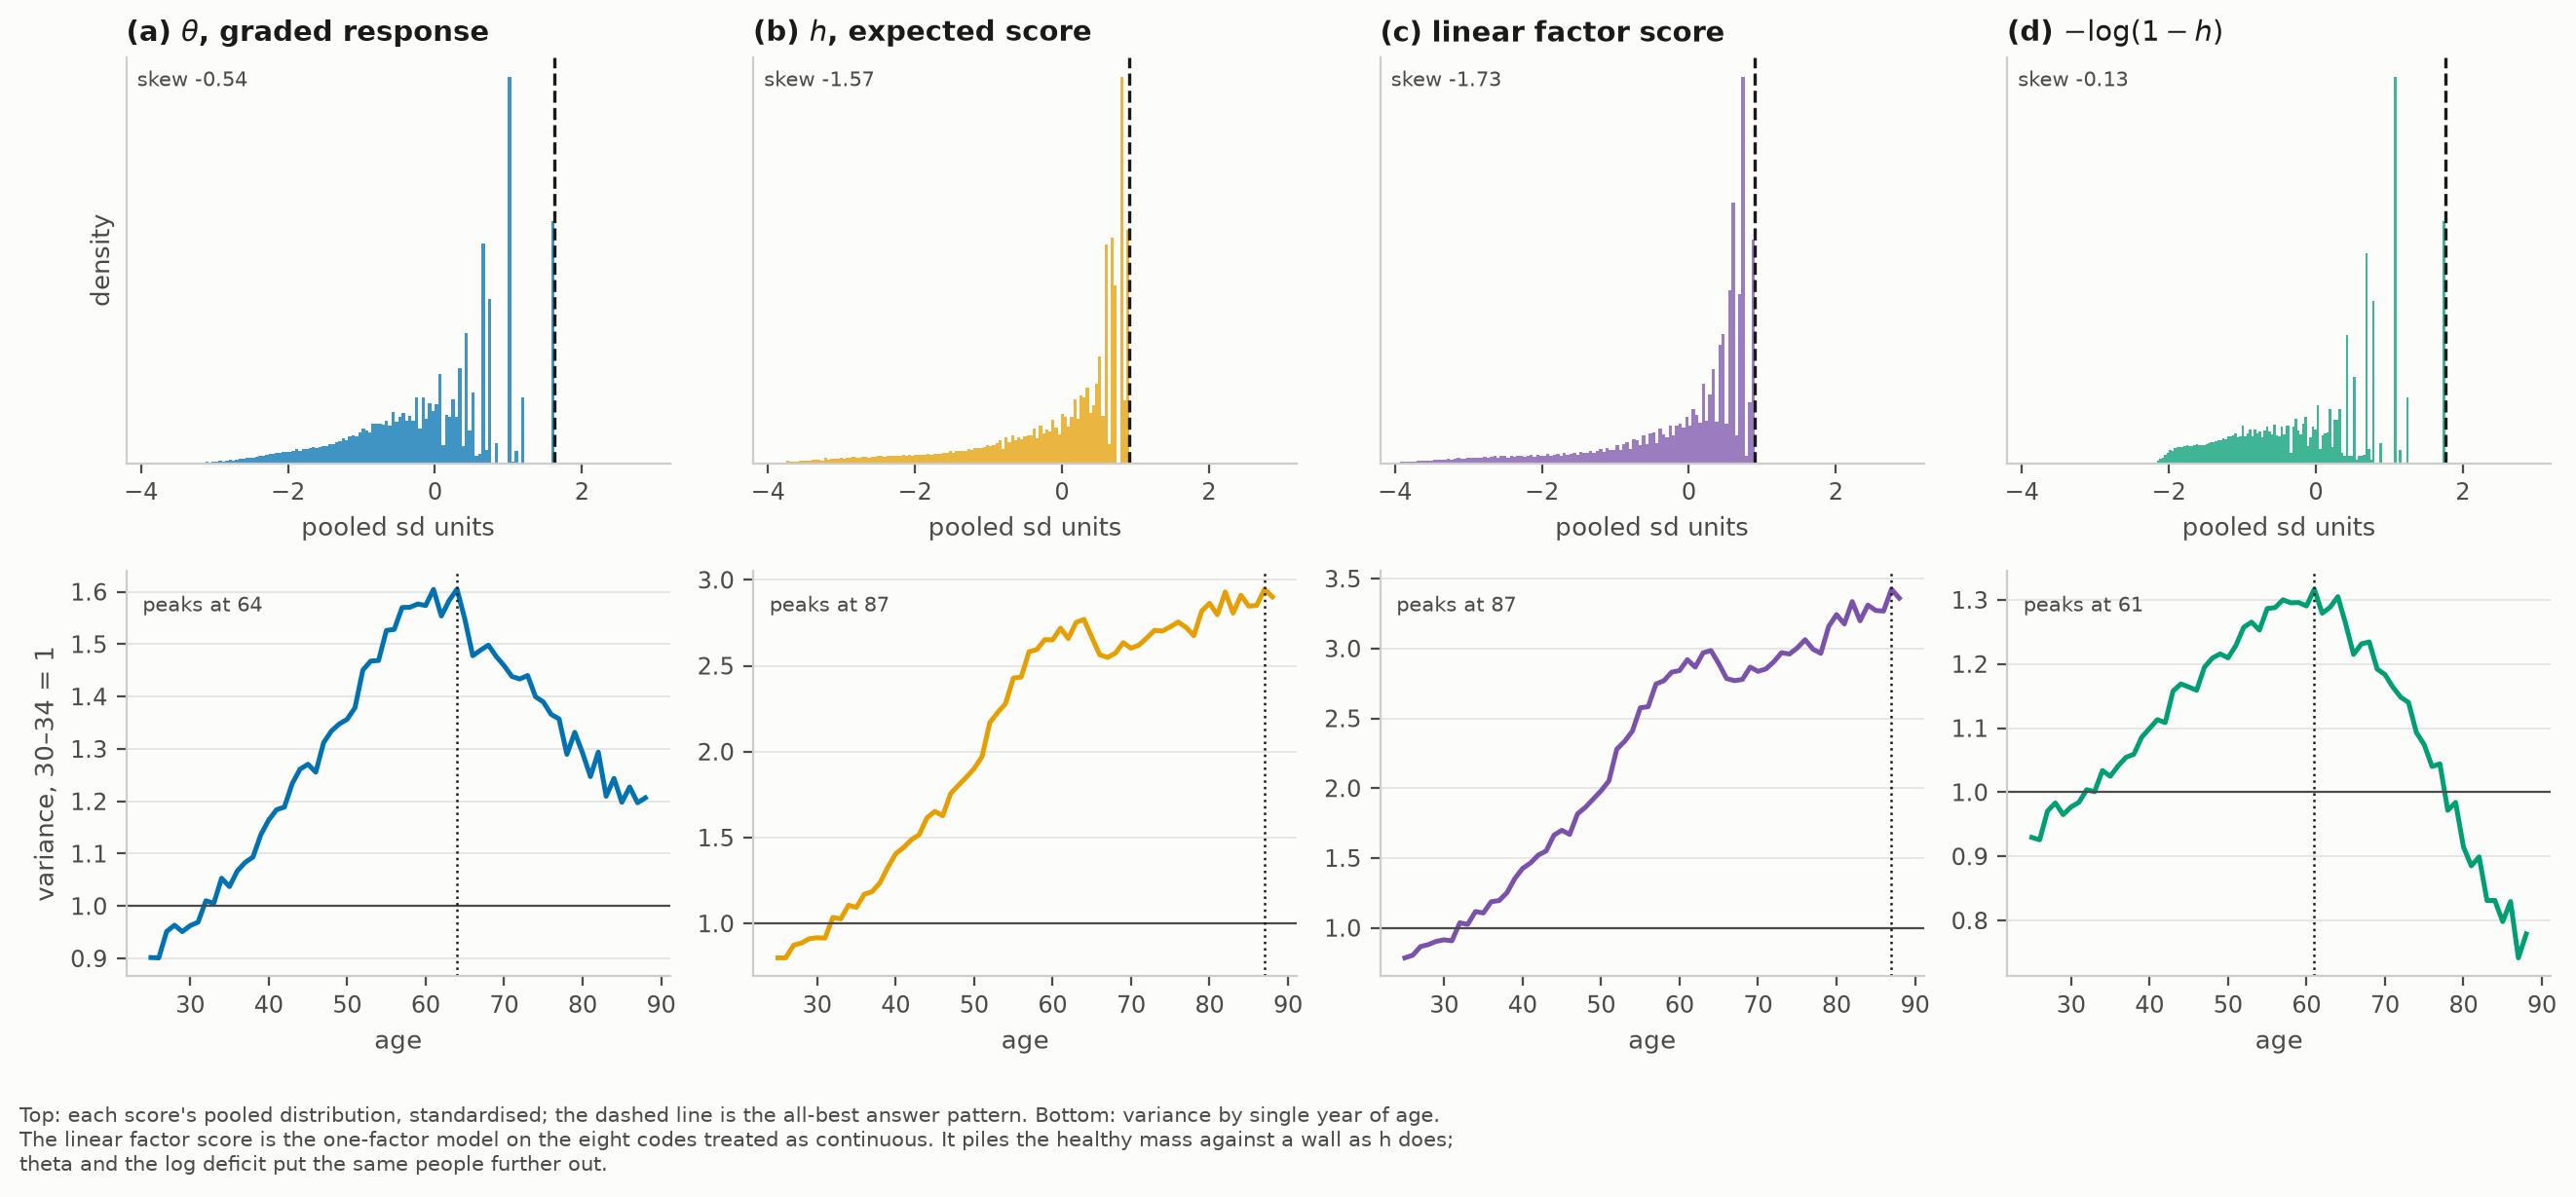
\includegraphics[width=\linewidth]{fig_health_factor}
\caption{The linear factor score against $\theta$ and $h$. Top: each score's pooled distribution, standardised, with the all-best answer pattern dashed. Bottom: variance by single year of age. The linear factor score piles the healthy mass against a wall as $h$ does; $\theta$ and the log deficit put the same people further out and their variance turns over in the early sixties.}
\label{fig:factor}
\end{figure}

\subsection{A simpler version reaches the same conclusions}

This was a requirement, not a bonus. The same eight variables, pooled three
ways --- the model's $\theta$, its $[0,1]$ transform, and an equal-weighted
deficit index --- agree on the floor, on continuity, on convexity, on the
variance rising up to 60, on mortality, on the sign path, and on
the two cost conclusions: convexity in pounds and age-invariance at fixed
health. What differs across them --- the size of per-standard-deviation
effects and the variance profile after 60 (Sections~\ref{sec:invariance}
and~\ref{sec:factor}) --- is a fact about cardinalisation that we state rather
than a disagreement about the world. The appendix weighted sum makes the same point inside the model:
$h$ is a weighted sum of the eight coded answers to $R^2 = 0.993$. A linear
factor model, the version an economist would fit without the graded-response
model, is a fourth pooling and agrees too (Section~\ref{sec:factor}): its
content is the same weighting, and on the scale-dependent properties it
lands with $h$.


\part{The cost index}

\section{What it is}
\label{sec:costwhat}

A per-person-wave estimate of annual NHS secondary-care cost, in a fixed price year, for waves 7--15, built from UKHLS alone. It is wrong in level and, on the evidence below, roughly right in \emph{shape}, which is what the framework needs: every question asked of it is about how cost varies with health, not about its absolute size. It is a secondary-care bed-day-weighted cost index and is named that way throughout, rather than called a cost.

The one-line target:
\[
  \widehat{C}_{it} \;=\;
  \underbrace{c_{\text{spell}}(k) + c_{\text{bed}} \cdot (\text{nights}_{it} - \bar{L})^{+}}_{\text{in-patient}}
  \;+\;
  \underbrace{c_{\text{op}} \cdot \widehat{n}^{\text{op}}_{it}}_{\text{out-patient}}
  \;+\;
  \underbrace{c_{\text{gp}} \cdot \widehat{n}^{\text{gp}}_{it}}_{\text{GP}}
\]
with $k$ the attributed condition where there is one, and everything indexed to a single price year.

\section{Ingredients}

\begin{center}\small
\begin{tabular}{llp{6.4cm}}
\toprule
Quantity & Source & Status \\
\midrule
Any admission & \code{hosp}, waves 7--15 & complete for respondents \\
Nights & \code{hospd} & all admitted; median 3, mean 7.5, max 300 \\
Maternity flag & \code{hospch} & 12.7\% of admissions, mean age 31.7 \\
Nights by new condition & \code{hospdc}$i$, waves 2--15 & 21\% of admissions \\
Nights by prior condition & \code{hospdcp}$i$, waves 11--15 & 11\% of admissions \\
\quad either & & 29\% of admissions, \textbf{65\% of nights} \\
\multicolumn{3}{l}{\footnotesize Attribution shares are for wave 15, the first wave carrying both questions.} \\
GP visits, banded & \code{hl2gp} & 0 / 1--2 / 3--5 / 6--10 / more than 10 \\
Out-patient attendances, banded & \code{hl2hop} & same bands \\
\bottomrule
\end{tabular}
\end{center}

UKHLS gives three tiers of contact, not two: \code{hl2gp} is ``Visited GP in last 12 months'' and \code{hl2hop} ``Hospital or clinic out-patient in last 12 months'', both banded $0$--$4$ across waves 7--15. (An earlier draft had the two swapped; the labels were re-checked directly in waves g, j and o.) Unit costs come from the NHS National Cost Collection, which publishes national average unit costs annually: non-elective in-patient episode about \pounds1{,}590, elective about \pounds3{,}684, day case about \pounds738, excess bed day about \pounds313, out-patient attendance about \pounds120.

\section{Construction}

\subsection{The flat-rate index}
Each admission is costed at the non-elective episode rate plus excess bed days beyond the average inclusive length of stay; out-patient attendances and GP visits at their flat rates, with band midpoints $0, 1.5, 4, 8, 15$. Maternity admissions are separable. At indicative unit costs the flat index averages \pounds539 per person-year: \pounds243 in-patient, \pounds182 out-patient, \pounds114 GP.

The one real modelling decision: UKHLS gives total nights but not the number of spells, so a person with 20 nights might have had one long admission or four short ones, which differ in cost by a factor of about three. The index assumes one spell; Section~\ref{sec:coststage4} tests how much that matters.

\subsection{Condition weighting}
For the nights carrying a condition attribution, the flat rate is replaced by a condition-specific one, mapping UKHLS condition code to NCC HRG chapter to average cost, at chapter level since the survey identifies a condition and not a procedure. Unattributed nights take the case-mix-weighted average of the attributed ones \emph{within the same decile of the health measure}, never a global average, which would flatten exactly the gradient the index is for. Attribution reaches 18.0\% of admissions pooled over waves 7--15, below the 29\% on wave 15 alone because \code{hospcp}/\code{hospdcp} begin at wave 11. Weighting moves the mean to \pounds566, about 6\%. More useful is what it does not do: the imputed condition weight is nearly flat across deciles of physical health, $1.16$ to $1.31$. Sicker people are not admitted for systematically more expensive conditions; they are admitted more often and for longer. Condition weighting is a level adjustment, not a shape one.

\section{Validation against published profiles}
\label{sec:costval}

The utilisation sample is $301{,}390$ person-waves on $59{,}750$ people, waves 7--15; the validation restricts to ages 20--90, $283{,}852$ person-waves. Three checks against what is independently known about NHS spending, none of which the index was fitted to.

\begin{figure}[H]
\centering

\includegraphics[width=\linewidth]{fig_cost_validation}
\caption{Validation of the flat-rate index. Panel (a) the age profile of the whole index and of each tier, relative to the 50s, against the published all-care ratio; (b) the share of each age band top-coded at ``more than ten'' contacts, with the top-band sensitivity; (c) the concentration curve against the published top-decile share; (d) the gradient in physical health, the quantity the index is for.}
\label{fig:costval}
\end{figure}

\begin{itemize}
\item \textbf{Concentration passes.} The top 1\% of person-waves hold 25.2\% of the total, the top 5\% 48.5\% and the top decile 65.6\%, against a published benchmark of more than half. If anything the index is over-concentrated, which is expected: 22.7\% of person-waves are exactly zero on an index that carries no prescribing, A\&E or community contact, the components that would give almost everyone a small positive amount.
\item \textbf{Level undershoots, as predicted.} \pounds539 per person-year against NHS spend per head near \pounds3{,}000. Three tiers of contact priced at national averages cannot add to the national total; the shortfall is not informative.
\item \textbf{The age profile strains.} The whole index puts the 80+ band at $2.5\times$ the 50s, against a published all-care ratio near $7\times$. By tier: in-patient $3.8\times$, out-patient $1.7\times$, GP $1.4\times$. The one tier measured as a true count is the one with a credible gradient; the two banded tiers are nearly flat in age. The bands are not the reason: top-coding does rise with age (7.4\% of the 80+ band at ``more than ten'' GP visits against 4.9\% of the 50s), but scoring the top band at 30 contacts rather than 15 moves the whole-index ratio from $2.47\times$ to $2.38\times$, the wrong way, because it loads more weight onto the tiers that are flat in age. The binding limitation is that cost per contact is held fixed: an out-patient attendance for an 85-year-old and one for a 30-year-old enter at the same \pounds120. That is what linkage to administrative records would fix.
\end{itemize}

\textbf{Verdict.} Usable for what it is for, with one stated caveat. The index's purpose is the gradient in \emph{health}, and there it is strong: $13.1\times$ between the least and most healthy decile on the whole index, $31.1\times$ on the in-patient tier, against an age gradient of $2.5\times$. The caveat is that the age profile is understated by roughly a factor of three, so the index should not be used for anything whose answer depends on the age gradient: lifetime cost projections, discounting, or the timing of prevention returns. For those, report the in-patient tier alone or wait for linkage.

\section{Convexity in pounds, and whether health matters more with age}
\label{sec:coststage4}

\begin{figure}[H]

\includegraphics[width=\linewidth]{fig_cost_convexity}
\caption{Cost index in pounds against five health measures: by decile, per standard deviation of each measure, and the sensitivity of the convexity to every costing assumption the index rests on. Measures oriented so higher means better health. Panel (c) varies the spell rule, maternity treatment, condition weighting and top-band value, each with a winsorised-at-the-99th-percentile twin.}
\label{fig:costconvex}
\end{figure}

\textbf{The costing assumptions do not matter, and neither does the health ruler for the sign.} All twelve variants of the sensitivity grid --- one spell, two spells, one per five nights; maternity in or out; flat or condition-weighted; top band at 15 or 30 --- are convex in pounds on the health measure's $\theta$, with person-clustered $t$ between $19$ and $39$. Winsorising at the 99th percentile halves the magnitude and changes nothing else; the sickest-to-healthiest ratio stays between $8.2\times$ and $14.4\times$. The spell ambiguity, which looked like the most damaging gap in the data, is not binding. Convexity also holds on every health measure in the figure: $h$, the UKHLS PCS, the SF-6D utility and the mental-health $\theta$, with the smallest $t$ at $10.3$. What the horizontal ruler sets is the size of the bend per standard deviation, not its sign: the quadratic term is \pounds201 on $\theta$ against \pounds113 on $h$, and \pounds106 against \pounds35 on capped costs.

\begin{figure}[H]

\includegraphics[width=\linewidth]{fig_cost_age_interaction}
\caption{The cost index in pounds against health within age bands. Panel (a) cost across pooled percentile bins of health, one line per age band; (b) the same table read down the other way; (c) the ratio of the sickest to the healthiest tenth; (d) the slope per standard deviation of $\theta$ and of $h$ over the full range; (e) the ratio of the oldest to the youngest band's slope within windows of the pooled distribution; (f) the share of each band falling in the sickest pooled tenth. Panels (a)--(c) and (f) are the same on every health scale.}
\label{fig:costage}
\end{figure}

\textbf{In pounds, the health--cost relationship is close to age-invariant on every ruler.} At a fixed level of health the index is nearly flat in age, shallow-U-shaped with a midlife minimum: the sickest tenth costs \pounds2{,}143 at 20--34 and \pounds2{,}136 at 75--90, and the sickest-to-healthiest ratio is $10$--$14\times$ at every age. The full-range gradient does rise, \pounds357 to \pounds741 per standard deviation of $\theta$ and \pounds526 to \pounds672 per standard deviation of $h$, but the pooled test with a quadratic in health finds no tilt: the health $\times$ age term is $-$\pounds4 per decade on $\theta$ ($t=-0.6$) and $-$\pounds2 on $h$ ($t=-0.3$). Ageing raises cost by moving people down a fixed curve, 2.5\% of the 20--34 band in the sickest pooled tenth against 24.7\% of the 75--90 band, not by changing its shape. Section~\ref{sec:invariance} has the full comparison across variants. Two cautions push the same way: the age profile is understated threefold, and UKHLS does not follow people into care homes, so the sickest old are under-represented in a way the sickest young are not.

\section{What the index cannot do}

Primary-care prescribing, A\&E and community services are absent entirely, and they are not a small share of NHS spend. Out-patient and GP use are four-band counts, so their intensive margins are crude. Elective and emergency admissions are indistinguishable, though they differ in cost by more than a factor of two. And every quantity is self-reported over a twelve-month recall window, against wave spacing that is not exactly twelve months. Linkage to hospital episode records (HES, through the UK Longitudinal Linkage Collaboration) would resolve the spell count, the case mix and the age profile at once; given that the convexity survives every costing assumption, it is a refinement rather than a precondition, and the binding risk is sample size, roughly $8{,}000$ consented participants against the $69{,}958$ people in the measure's sample.

\part*{Reproducing it}
\section{Reproducing it}

\begin{center}\small
\begin{tabular}{p{7.1cm}p{7.6cm}}
\toprule
\code{data\_cleaning/01\_build\_panel.py} & the processed UKHLS panel \\
\code{02\_build\_measures.py} & the SF-12 item extract every later step reads \\
\code{03\_build\_chronic.py} & condition histories \\
\code{04\_build\_health.py} & \textbf{the measure}: \code{health\_measure.parquet} with \code{theta}, \code{theta\_sd}, \code{h}, \code{fi10}, \code{ws}, plus item, $Q_3$, age-profile and weight tables \\
\code{05\_build\_cost\_proxy.py} & \textbf{the cost index}: \code{cost\_index.parquet}, flat-rate and condition-weighted \\
\code{descriptives/21\_health\_measure.py} & Part~I's figures and properties table, the pound gradients by age of Section~\ref{sec:invariance}, and the linear factor comparison of Section~\ref{sec:factor} \\
\code{descriptives/24\_paper\_measure\_tables.py} & correlations with the PCS, MCS and condition count, and mortality \\
\code{descriptives/15\_cost\_validation.py} & the validation of Section~\ref{sec:costval} \\
\code{descriptives/16\_cost\_convexity.py}, \code{17\_cost\_age\_interaction.py} & Section~\ref{sec:coststage4}: convexity in pounds, the costing sensitivity, the age interaction \\
\bottomrule
\end{tabular}
\end{center}

The bank, the coding rules and the deficit index live in
\code{measures/health.py}, so anything that needs the measure's definition
imports it rather than re-deriving it. \code{04\_build\_health.py} gates every
run on: no positive local dependence, the EAP identity
$\mathrm{Var}(\theta) + \overline{\mathrm{SE}^2} = 1$ (it holds to three
decimals), the three variants agreeing in rank, and exact reproduction of the
search's P-LIM3+CC scores while those outputs are still on disk. Outputs derive
from licensed UKHLS microdata and are gitignored.

\appendix

\section{The weighted sum behind $h$}
\label{sec:weights}

Regressing $h$ on the eight standardised category codes gives $R^2 = 0.993$
(387,599 person-waves). Normalised to sum to one, the weights are:

\begin{center}\small
\begin{tabular}{lrrrrrrrr}
\toprule
& GH & PF & RP & BP & LIM\_FL & LIM\_SELF & LIM\_SENS & COND \\
\midrule
weight (\%) & 13.1 & 22.1 & 22.0 & 13.5 & 15.2 & 5.4 & 2.5 & 6.3 \\
\bottomrule
\end{tabular}
\end{center}

This is not a coincidence of this sample. In the ordinal factor model that the
graded-response model is a reparameterisation of, the loading is
$\lambda_j = a_j/\sqrt{a_j^2 + 1.702^2}$ and the optimal score weights are
proportional to $\lambda_j/\psi_j$ --- so a graded-response score is, to a very
good approximation, a weighted sum whose weights the data chose. The practical
content of the model is therefore the \emph{weights}, not the functional form:
it puts 71\% on the SF-12 testlets, 23\% on the impairment groups and 6\% on
diagnoses, where \code{fi10} puts 60\%, 30\% and 10\%. That the two give the same answers (Spearman $0.991$) is what
makes the model defensible to an audience that does not want one.

How good the approximation is depends on which variant is being approximated, and
the ordering is worth stating because the dynamic models default to $\theta$:

\begin{center}\small
\begin{tabular}{lrl}
\toprule
Variant & $R^2$ on the eight codes & \\
\midrule
\code{fi10} & $1.000$ & exact: every deficit is affine in a code \\
$h$ & $0.993$ & the expected-score curve nearly undoes the {EAP} nonlinearity \\
$\theta$ & $0.925$ & the posterior mean stretches the tails \\
\bottomrule
\end{tabular}
\end{center}

The deficit index is exactly a weighted sum because each of its ten deficits is an
affine function of one of the eight codes, with the caps never binding: the
two physical-function items sum to the {PF} testlet, the two role items to {RP},
each impairment share is its count over a fixed number of areas, and the
condition deficit and the {COND} code are both the count capped at six. $h$ is
close to one because the expected-score curve is nearly the inverse of the map
from pattern to $\theta$: $h$ is an expected raw score, and a raw score is a sum
of codes. $\theta$ is furthest because it is the posterior mean, which pushes
extreme patterns further out than any linear index can follow. The weighted-sum
defence of the model is therefore strongest exactly where the paper uses the
bounded scale, and weakest on the latent scale that is the mixtures' default.

\section{Relation to what is used elsewhere}

The SF-12 physical component summary is itself a weighted sum of these items,
with regression weights chosen in a US general-population sample to reproduce the SF-36
summaries \citep{ware1996}, whose orthogonal factor structure gives each summary weights
on the other domain's items \citep{farivar2007}; the archived note documents a 6.6-point artifact at the
median physical profile that follows from that mixing. The graded-response
approach differs in three ways: the weights are estimated on this sample, the
mental items are absent by construction, and the scale is a latent one rather
than a linear combination with an arbitrary origin.

Item-response measurement of physical function is standard in the health
measurement literature \citep[PROMIS physical function;][]{cella2010} and
deficit accumulation is standard in the frailty literature \citep{mitnitski2001,searle2008}; the combination of
SF-12 items with impairment counts and a diagnosis count is ours, and is
documented here rather than borrowed. In economics the closest relatives are
the health indices built by factor methods from panel surveys --- the point of
appendix~\ref{sec:weights} is that a reader who prefers that tradition can read
our measure as one of those, with weights in a table, and lose nothing.

\bibliographystyle{plainnat}
\bibliography{references}

\end{document}
